\section{Passive-Aggressive with Bandit feedback (PAB)}
In the previous section, we have introduced the multiclass classification algorithm with Bandit feedback, i.e. Banditron, Confidit. Here, we present a novel algorithm PAB\cite{zhong2015esann} in Algorithm~\ref{algo:pab}, which is an adaptation of PA for the bandit case. 

Similar to PA algorithm, at each round the prediction $\hat{y}_t$ is chosen by Bayesian 
probability according to the current weight matrix $w_t$, to make a reference to Eq(\ref{equa:prediction}).
%\[\hat{y}_t = \underset{i \in [k]}{argmax} <w_t, \Phi(x_t,i)>\]
%Most of time, the PAB exploits the quality of the current weight matrix by predicting the label. 
Unlike the conventional learning paradigm, if $\hat{y}_t \neq y_t$, it needs to perform an \emph{exploration}, i.e sample a label 
randomly from [k] with parameter $\gamma$ and contrast this random prediction with a bandit return $\1(\tilde{y}_t=y_t)$, 
where $\tilde{y}_t$ is the result of a random draw from a certain distribution $\mathbb{P}(\tilde{Y}|\hat{y})$.
%If $\tilde{y}_t = y_t$, it means we obtain the  identity of $y_t$ by chance.

The above intuitive argument is formalized by defining the update 
matrix $\tilde{U}_t$ to be a function of the random prediction $\tilde{y}_t$. We  show in the following 
that the expectation of the PAB's update is exactly the PA's update.

PAB starts with the initiation of matrix $w_1 = \boldsymbol{0}$. Its update contains two items:
\begin{equation}\label{eq:PAB}
\begin{split}
&w_{t+1}=w_t+U_{PAB}(x_t,\hat{y}_t,\tilde{y}_t) = w_t + U_{t,1} + U_{t,2}\\
&U_{t,1} =\frac{\1(\tilde{y}_t = y_t)}{\mathbb{P}(\tilde{Y}=\tilde{y}_t|\hat{y}_t)}U_{PA}(x_t,\hat{y}_t,\tilde{y}_t) \\
&U_{t,2} =\frac{\1(\tilde{y}_t = y_t)- \mathbb{P}(\tilde{Y} =\tilde{y}_t|\hat{y}_t)}{\mathbb{P}(\tilde{Y}=\tilde{y}_t|\hat{y}_t)}\cdot \rho_c \frac{\Phi(x_t,\hat{y_t})}{2\parallel{x_t}\parallel^2+\frac{1}{2C}}\\
\end{split}
\end{equation}
where $U_{PA}(x,\hat{y},y)$ is the classical passive-agressive update. 
PAB's update contains two items. The first item is controlled by the indicator $\1(\tilde{y}_t=y_t)$, 
and is nonzero only when the true label is predicted. 
The role of second term is to smooth the learning process when few correct labels are available.
%To the loss function, the algorithm's goal is to achieve a margin at least $\rho$ 
%as often as possible. On rounds where the algorithm attains a margin less than $\rho$ it suffers an instantaneous loss. 
It means that whenever the process is blind to the true label, the loss is estimated to a fixed number $\rho_c$;
this parameter is chosen empirically.

%\newtheorem{lemma}{Lemma}

\subsection{Simple PAB}
\label{subsec:SPAB}
A simple choice is $\rho_c = 0$. 
The item $U_{t,1}$ is very similar to the PA's update. The following lemma is easy to prove:
\begin{lema} 
\label{lema:pab1}
Let $U_{t,1}$ be  defined as in eq.(\ref{eq:PAB}) and let $U_{PA}(x_t,\hat{y}_t,y_t)$ 
be defined according to eq.(\ref{equa:paupdate}). Then, $\mathbb{E}_{\tilde{Y}}[U_{t,1}]=U_{PA}(x_t,\hat{y}_t,y_t)$.
\end{lema}
\begin{proof}
\begin{align*}
\mathbb{E}_{\tilde{Y}}[U_{t,1}] &= \sum_{i=1}^{k}  \mathbb{P}(i|\hat{y})\cdot U_{t,1}\\
&=\sum_{i=1}^{k}\mathbb{P}(i|\hat{y})\1(i=y_t)\frac{U_{PA}(x_t,\hat{y}_t,i)}{\mathbb{P}(i|\hat{y})}\\
&=\sum_{i=1}^{k} \1(i=y_t)U_{PA}(x_t,\hat{y}_t,i) \\
&=U_{PA}(x_t,\hat{y}_t,y_t)
\end{align*}
\end{proof}
By the way, simple PAB is much easy and quick to learn data, also good enough to deal with the synthetic data by the expectation $U_{PA}$. 

\subsection{Full PAB}
\label{subsec:FPAB}
Without item $U_{t,2}$,  $\tilde{U}$ behaves like the $U_{PA}$, when $\tilde{y}_t = y_t$ . 
And it works very well with some linear data, but it's poor to learn data real and noisy. By this appearance, we get  the importance of item  
The second term $U_{t,2}$ is used to reduce the variance of the update.
When $\rho_c > 0$, we need both $\mathbb{E}_{\tilde{Y}}[U_{t,2}] = 0$ (so that $\mathbb{E}_{\tilde{Y}}[{U}_{PAB}(x_t,\hat{y}_t,\tilde{Y})] = U_{PA}(x_t,\hat{y}_t,y_t))$) and  $\mathbb{E}_{\tilde{Y}}[<U_{t,1},U_{t,2}>] \leq 0$.  
%We have some experiments to compare it with others algorithm, also with the simple PAB. The results could be seen in section 4 Experiments.

\begin{lema} 
\label{lema:pab2}
Let $U_{t,2}$ be defined as in eq.(\ref{eq:PAB}),  $\mathbb{E}_{\tilde{Y}}[U_{t,2}]=0$.
\end{lema}

\begin{proof}
For each round t, we have
\[
\begin{split}
\mathbb{E}_{\tilde{Y}}[U_{t,2}] &= \sum_{i=1}^{k} \mathbb{P}(i|\hat{y}_t)\cdot U_{t,2} \\
&= \sum_{i=1}^{k}\mathbb{P}(i|\hat{y}_t)\frac{\mathbb{I}(i=y_t)-\mathbb{P}(i|\hat{y}_t)}{\mathbb{P}(i|\hat{y}_t)}\frac{\rho_c}{2\parallel{x}\parallel^2+\frac{1}{2C}}\Phi(x_t,\hat{y}_t)\\
&= \sum_{i=1}^{k}(\mathbb{I}(i=y_t)-\mathbb{P}(i|\hat{y}_t))\frac{\rho_c}{2\parallel{x}\parallel^2+\frac{1}{2C}}\Phi(x_t,\hat{y}_t) \\
&= (1-\mathbb{P}(y_t|\hat{y}))\frac{\rho_c}{2\parallel{x}\parallel^2+\frac{1}{2C}}\Phi(x_t,\hat{y}_t)\\
&-\underset{i\neq y_t}{\sum} \mathbb{P}(i|\hat{y}_t)\frac{\rho}{2\parallel{x}\parallel^2+\frac{1}{2C}}\Phi(x_t,\hat{y}_t)\\
& =0.
\end{split}
\]
\end{proof}
\begin{lema}
\label{lema:pab3}
$\mathbb{E}_{\tilde{Y}}[<U_{t,1},U_{t,2}>]  \leq 0$
\end{lema}
\begin{proof}
\[
\begin{split}
\mathbb{E}_{\tilde{Y}}[<U_{t,1},U_{t,2}>]  
&= \sum_{i=1}^{k} \mathbb{P}(i|\hat{y}_t)\mathbb{I}(i=y_t)\frac{U_{PA}(\hat{y}_t)}{\mathbb{P}(i|\hat{y}_t)} \frac{\1(i=y_t)-\mathbb{P}(i|\hat{y}_t)}{\mathbb{P}(i|\hat{y})}\frac{\rho_c \Phi(x_t,\hat{y}_t)}{2\parallel{x}\parallel^2+\frac{1}{2C}} \\
&= \frac{1-\mathbb{P}(y_t|\hat{y}_t)}{\mathbb{P}(y_t|\hat{y}_t)}\rho_c f(x_t, \hat{y}_t,y_t)
\end{split}
\]
with
\[f(x_t,\hat{y}_t,y_t) = \frac{<U_{PA}(x_t,\hat{y}_t,y_t),\Phi(x_t,\hat{y}_t)>}{2\parallel{x}\parallel^2+\frac{1}{2C}}\]
then:

\[\mathbb{E}_{\tilde{Y}}[<U_{t,1},U_{t,2}>] = \1(\hat{y}_t=y_t) \frac{1-\mathbb{P}(\tilde{Y}=y_t|\hat{y}_t)}{\mathbb{P}(\tilde{Y}=y_t|\hat{y}_t)}\rho_cf(x_t,\hat{y}_t,y_t)+ \1(\hat{y}_t \neq y_t) \frac{1-\mathbb{P}(\tilde{Y}=y_t|\hat{y}_t)}{\mathbb{P}(\tilde{Y}=y_t|\hat{y}_t)}\rho_cf(x_t,\hat{y}_t,y_t)\]

When $\hat{y}_t = y_t $, $U_{PA} = 0$ so that $f(x_t,\hat{y}_t,y_t)=0$.  When $\hat{y}_t \neq y_t $, it can be shown  that $f(x_t,\hat{y}_t,y_t)\leq 0$, so that:

\[
\mathbb{E}_{\tilde{Y}}[<U_t^1,U_t^2>] \leq 0
\]
\end{proof}
For an appropriate value of $\rho_c$, the role of $U_{t,2}$ is thus  to \emph{reduce} the variance of the PAB update,
and thus improve the speed of the learning process.
%So with the item $U_{t,2}$, PAB has more capacity than the simple PAB, also be more complex.

%%%%%%%%%%%%%%%%%%%%%%%%%%
\begin{algo}[PAB]
\label{algo:pab}
\begin{algorithmic}
   \STATE $\ \ $
	\STATE   Initiation $w_1=\vec 0$.
	\FOR	{for each instance $t=1,2,...,T $}
	\STATE   Receive $\xt\in \Rd$
	\STATE   Set $\hy= \underset{r\in \{1,\dots,K\}}{\text{argmax}}(W_t \Phi(x_t,r))$    
    \[\forall i \in [k], \mathbb{P}(\tY = i|\hy)=\1 (\hy=i)\cdot \epsilon+\frac{\epsilon}{k}\]	
	\STATE    Randomly sample $\ty$ according to $\mathbb{P}(\tY=i|\hy)$
	\STATE	 Receive the feedback $\1(\tilde{y}_t=y_t)$
   \[ l_t = < w_t,\Phi(x_t,\hat{y}_t)-\Phi(x_t,y_t) >+ \1(\hat{y}_t = y_t)\]
 \[U_{t,1} =\frac{\1(\tilde{y}_t = y_t)}{\mathbb{P}(\tilde{Y}=\tilde{y}_t|\hat{y}_t)}U_{PA}(x_t,\hat{y}_t,\tilde{y}_t) \]
\[U_{t,2} =\frac{\1(\tilde{y}_t = y_t)- \mathbb{P}(\tilde{Y} =\tilde{y}_t|\hat{y}_t)}{\mathbb{P}(\tilde{Y} =\tilde{y}_t|\hat{y}_t)}\cdot \frac{\rho_c}{2\parallel{x_t}\parallel^2+\frac{1}{2C}}\Phi(x_t,\hat{y_t})\]
\[U_{PAB,t}(x_t,\hat{y}_t,\tilde{y}_t) = U_{t,1} + U_{t,2}\]
	\STATE	Update:$W_{t+1}=W_t+U_{PAB,t}(x_t,\hat{y}_t,\tilde{y}_t)$
    \ENDFOR
\end{algorithmic}
\end{algo}
%%%%%%%%%%%%%%%%%%%%%%%
\subsection{Experiments}
\label{subsec:EPAB}
In this section, we present experimental results for the PAB and other bandit algorithms on two synthetic and one real world data sets. The cumulative loss is presented for each data set.

The first data set, denoted by SynSep, is a 9-classes, 400-dimensional synthetic data set of size $10^5$. The method to generate the sample is found in \cite{kakade2008efficient}. The second data set, denoted by SynNonSep, is constructed in the same way as SynSep except that a $5\%$ label noise is added, which makes the data set non-separable. The third data set is collected from the Reuters RCV1 collection. This set is made of 47236-dimensional vectors, contains 4 classes (to choose the first level categorization.) with the size of $10^5$.

In the Figure~\ref{pic:PABSynSep} gives the cumulative loss obtained on the dataset SynSep for different online learning algorithm. Here, the Confidit algorithm (see in Appendix~\ref{algo:confidit}) provides the best results, but the Simple PAB takes the second. Three out of five algorithms attain a zero loss. The worst in that case is the Banditron (see in Appendix~\ref{algo:banditron}). 

\begin{figure}[!h]
\vspace{.2in}
\centering{
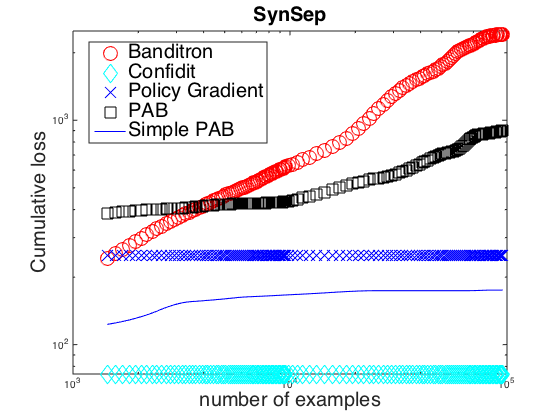
\includegraphics[scale = 0.6]{chapters/chapter05/fig05/mc/PAB_SynSep.png}}
\caption{Cumulative loss of each algorithm under the SynSep data. Parameters: $\gamma = 0.014$ for Banditron, $\alpha=1$, $\eta=1000$ for Confidit, $\eta =0.01$, $\lambda = 0.001$ for Policy Gradient; $C = 0.001$, $\gamma = 0.7$ and $\rho = 0$ for Simple PAB, $\rho = 1$ for Full PAB.}
\label{pic:PABSynSep}
\end{figure} 

In the Figure~\ref{pic:PABSynNonSep}, it shows the result on the SynNonSep data set, the results are rather poor in general. The Confidit and Policy Gradient \cite{Dauce13fast} obtain the best performances, with a stable final error rate around $5\%$. 
\begin{figure}[!h]
\vspace{.2in}
\centering{
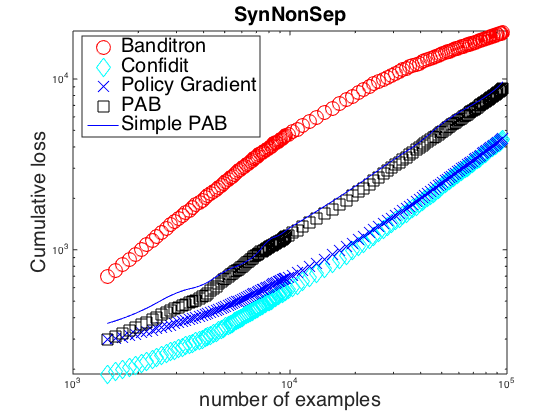
\includegraphics[scale = 0.6]{chapters/chapter05/fig05/mc/PAB_SynNonSep.png}}
\caption{Cumulative loss of each algorithm under the SynNonSep data. Parameters: $\gamma = 0.006$ for Banditron, $\alpha=1$, $\eta=1000$ for Confidit, $\eta =0.01$, $\lambda = 0.001$ for Policy Gradient; $C = 0.00001$, $\gamma = 0.7$ and $\rho = 0$ for Simple PAB, $\rho = 1$ for Full PAB.}
\label{pic:PABSynNonSep}
\end{figure}

In the Figure~\ref{pic:PABRCV}, it's on the Reuters data with the first level categorization. On contrast with the synthetic datasets, the full PAB overtakes the other methods, with a final error rate around $2.5\%$ while the other algorithms attain $5\%$ error, and even worse in the case of Confidit ($8\%$ error rate). Besides, the PAB error rate is constantly reducing during the learning process.
\begin{figure}[!h]
\vspace{.2in}
\centering{
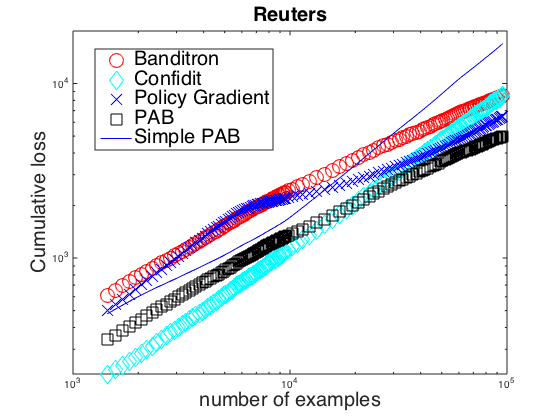
\includegraphics[scale = 0.6]{chapters/chapter05/fig05/mc/PAB_Reuters.png}}
\caption{Cumulative loss of each algorithm. Parameters: $\gamma = 0.05$ for Banditron, $\alpha=1$, $\eta=100$ for Confidit, $\eta =0.1$, $\lambda = 0.001$ for Policy Gradient; $C = 0.0001$, $\gamma = 0.6$ and $\rho = 0$ for Simple PAB, $\rho = 1$ for Full PAB.}
\label{pic:PABRCV}
\end{figure}

\subsection{Conclusion}
With the advantage of the Passive-Aggressive max-margin principle, the simple and full PAB appear effective to address the bandit online learning setting. Their first advantage is their linear complexity in space that allows to treat high dimensional datasets on the contrary to second-order methods. On separable data samples, the basic PAB overtakes most of the other approaches, at the exception of the Confidit algorithm, with a much lower complexity. It is however found to perform rather poorly on noisy and real world datasets. In contrast, the full PAB is expected to vary more smoothly over time, and is found to perform particularly well on the Reuters dataset. In that case, Confidit and Policy Gradient seem to fall in a local stable solution, while the full PAB constantly improves, issuing a better classifier.
However, the performance of the algorithm is found to depend on three free parameters $\gamma$, $\rho_c$ and $C$. In order to avoid fastidious cross-validation, additional investigation is needed in order to find analytic estimates of their optimal values. 